\documentclass{article}

\usepackage{amsfonts}

\usepackage{graphicx}
\graphicspath{ {./images/} }

\usepackage{bm}



\usepackage{amsmath}

\usepackage[a4paper, total={6in, 8in}]{geometry}


\setlength{\parindent}{0pt} % for getting rid of first line indentation


% ================================================
% =====================  BEGIN DOCUMENT 
% ================================================

\title{Game Theory Project}
\author{Juan Pablo Bello Gonzalez}
\date{September 2024}

\begin{document}

\maketitle

\newpage




\section{Introduction}

Counterfactual regret minimization (CFR) has become a leading algorithm for computing approximate Nash equilibria in imperfect information games, where players lack full knowledge of the game state. Poker, perhaps the most iconic example of such games, has served as a proving ground for CFR. Variants of the algorithm form the foundation of modern poker bots, some of which have achieved the remarkable feat of defeating professional players. This accomplishment is particularly impressive given the immense number of possible game states in poker.  

This paper examines how extensive form games can be used to model imperfect information scenarios and explores the CFR algorithm as introduced in \textit{Regret Minimization in Games with Incomplete Information} by Martin Zinkevich and collaborators. The implementation is demonstrated on Kuhn Poker, the simplest variant of poker, providing a foundation for understanding its broader and more computationally intensive applications.


\subsection{Khun Poker}

Kuhn Poker is a simplified two-player variant of poker designed to study strategic decision-making in games with imperfect information. Each player is dealt one card from a deck of three cards (\(J, Q, K\)), and the remaining card is hidden. Players then take turns deciding whether to check, bet, call, or fold based on their private card and the observed actions of their opponent. In the game, bets consist of one unit of utility for simplicity. The game has a zero-sum payoff structure, where one player's gain equals the other's loss, and the winner is determined by either a showdown or a fold. Despite its simplicity, Kuhn Poker captures key elements of poker, such as bluffing, information asymmetry, and strategic betting, making it a valuable model for exploring game theory concepts. Throughout this paper we will use the game of Kuhn poker to illustrate the concepts. 


\section{Extensive form games}

Extensive form games provide a framework for modelling sequential games, where players make decisions in a specific order, and utilities are distributed only at the game's conclusion. These games have a natural tree representation, with each node corresponding to a decision point for a player and branches representing the available actions. The tree alternates between players at each level, capturing the sequence of decisions and possible outcomes. Terminal nodes, or leaves, represent the end of the game, where payoffs are assigned based on the sequence of actions taken. This structure makes extensive form games particularly suited for modelling games like poker, where players act in turns, and the final utilities depend on the entire sequence of decisions made throughout the game ((((YOUTUBE))). Figure 1 displays the full tree representation of Kuhn Poker:

%%% IMAGE
\begin{figure}
    \centering
    \textbf{Figure 1}\par\medskip
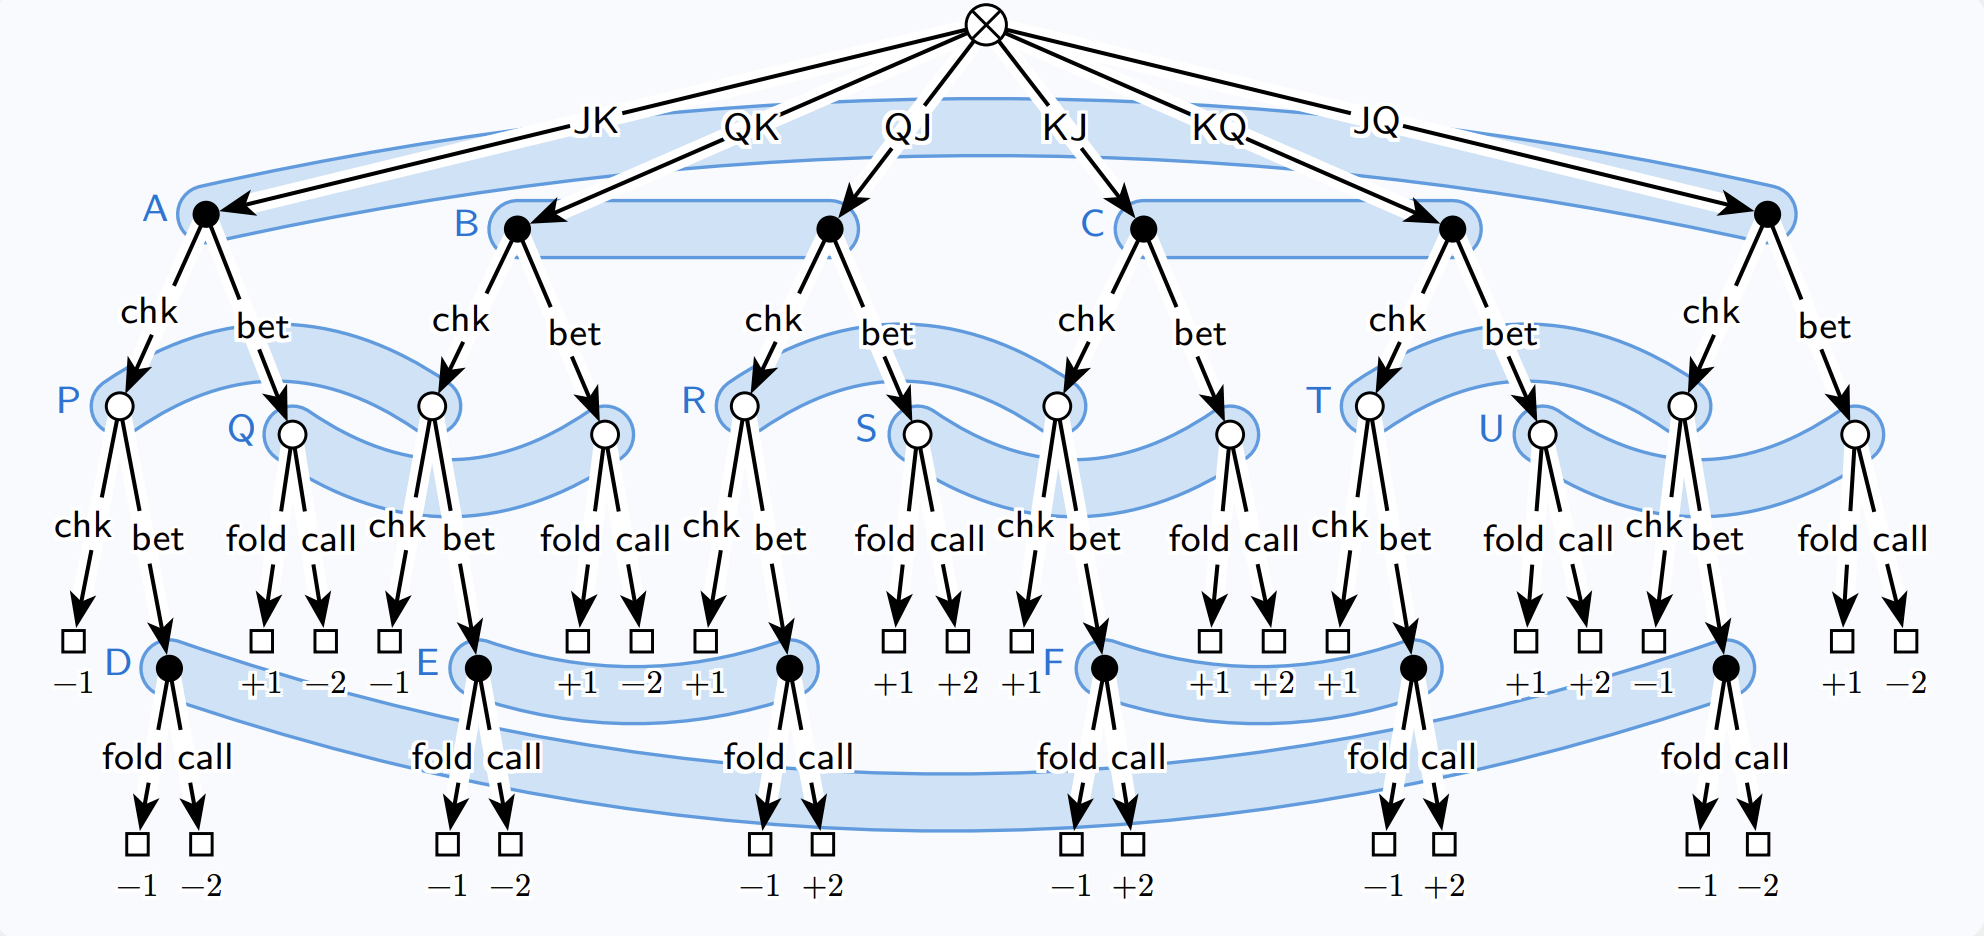
\includegraphics[scale=.44]{game_tree}
    \caption{Game tree of Kuhn Poker ((((MIT))))}
\end{figure}


\subsection{Imperfect Information}
Imperfect information games are games in which players do not have complete knowledge of all aspects of the game state, such as the actions or private information of other players. This contrasts with perfect information games, where every player is fully aware of the entire history and current state of the game at all times. Classic examples of perfect information games include chess and tic-tac-toe, where every move is visible to all players. In contrast, games like poker involve hidden information like private cards and undisclosed strategies, making them far more complex to analyze. This hidden information introduces uncertainty and requires players to reason about probabilities, hidden strategies, and the potential knowledge of their opponents. The study of imperfect information games is crucial in fields like game theory, artificial intelligence, and economics, as it mirrors real-world decision-making scenarios where perfect knowledge is rarely available.

To model imperfect information in extensive form games, we use \textbf{information sets}, which are groups of game states (or nodes in the game tree) that a player cannot distinguish between when making a decision. Each information set represents the player's uncertainty about the game's exact state at a given point. For example, in Kuhn Poker, Player 1 has three information sets at the first decision level, corresponding to the card they were dealt. If Player 1 is dealt a Jack, their information set is \( I_1 = \{JQ, JK\} \), reflecting uncertainty about whether Player 2 holds a Queen or a King. Similarly, if Player 1 is dealt a Queen, the information set is \( I_2 = \{QJ, QK\} \), and if dealt a King, it is \( I_3 = \{KJ, KQ\} \). These information sets capture both the card Player 1 holds and the hidden information about Player 2’s card.


\subsection{Formalizing Extensive Form Games}

According to (Zinkevich), a formal definition of an extensive game includes the following:

\begin{itemize}
\item A finite \textbf{set of players} $N$
\item A finite set of ordered action \textbf{histories} $H$, such that the empty sequence is in H and every prefix of a sequence in H is also in H. 
\begin{itemize}
\item Denote $Z \subseteq H$ as the set of terminal histories, corresponding to the leaves of the tree representation, where the game ends, it is no one's turn, and players receive their utilities.
\item Denote $A(h) = \{ a : (h,a) \in H \setminus Z\}$ as the actions available for the player whose turn it is after a non-terminal history $h \in H \setminus Z$.
\end{itemize}

\item A \textbf{player function}, $P: H \setminus Z \rightarrow N$ that specifies the player whose turn it is to act at the end of a given history.

\item A function $f_i$ that assigns, to every history $h$ where it is player $i$'s turn ($P(h) = i$), a probability measure over the possible actions $A(h)$ at that history. Specifically, $f_i(a|h)$ denotes the probability of player $i$ choosing action $a$ given $h$, with each such probability measure being independent of all others.


\item For each player $i \in N$ define their \textbf{information partition}, $\mathcal{I}_i$, as a partition of the set of histories where player $i$ is required to act, $\{ h \in H : P(h) = i \}$. Each member of the partition $I_i \ in \mathcal{I}_i$ is called an information set and it 
represents the subset of histories indistinguishable to player $i$, based on the information available to them at a specific point in time.

Information sets have the property that for all $h, h' \in I_i$, the available actions must be the same, i.e., $A(h) = A(h')$. 
\item For each player $i \in N$ define a utility function $u_i: Z \rightarrow \mathbb{R}$ that assigns a real-valued utility to each terminal state $z \in Z$. In extensive form games, player actions may occur at various points in time throughout the game, but utilities are assigned exclusively at the terminal states.
\end{itemize}


\section{Kuhn Poker as an extensive form game}
In the case of Kuhn poker, there are two players $N = \{1,2 \}$. To define the set of histories $H$, one can conceptualize the game as evolving through levels of the game tree: \\



\textbf{Level 0 (Root Node):}
\begin{itemize}
\item At time 0, nature deals one card to each player from the set $\{J, Q, K \}$.
\item The set of possible cards dealt is $\text{CARDS}  = \{ (c_1, c_2) : c_1, c_2 \in \{J, Q, K \}, c_1 \neq c_2 \}$.
\end{itemize}

\textbf{Level 1:}
\begin{itemize}
\item Player 1, knowing their card but not Player 2's, takes an action.
\item The actions available to Player 1 are $A_1 = \{\text{CHECK}, \text{BET}\}$.
\end{itemize}
\textbf{Level 2:}
\begin{itemize}
\item Player 2 responds to Player 1's action. 
\item The actions available depend on Player 1's choice:
If Player 1 CHECKS, Player 2 can choose: $\{ \text{CHECK}, \text{BET} \}$. If Player 1 BETS, Player 2 can choose $\{ \text{FOLD}, \text{CALL} \}$. So, in general, Player 2's first action at level 2 is from the union of these two sets, $A_2 = \{\text{CHECK}, \text{BET}, \text{FOLD}, \text{CALL} \}$ 
\end{itemize}
\textbf{Level 3:} 
\begin{itemize}
\item If the game continues (i.e., Player 2 bet as a response to Player 1 checking first), Player 1 has the final decision: $A_3 = \text{FOLD}, \text{CALL}$.
\end{itemize}

So, $H$ has the form: 

\[ H \subseteq \text{CARDS} \times A_1 \times A_2 \times A_3 \]

Some example histories are: Q.K.BET.FOLD, K.J.BET.CALL, and K.J.CHECK.BET.CALL. Note that the histories alternate players, so $P(h)= 1$ for histories $h$ of even length such as $Q.K$ and $Q.K.CHECK.BET$. Similarly, $P(h) = 2$ for histories of odd length such as $Q.K.BET$.

Histories also show complete information. Players themselves are not able to see histories, only their respective information sets. 

Each player has 6 information sets. The information sets for player 1 are labelled A-F on \textbf{Figure 1} and those of Player 2 are labelled  P-U. 


\subsubsection{Strategies}
In extensive form games, a strategy profile $\sigma$ is a complete contingent plan for each player $\sigma_i$ that specifies how a player will act at every possible decision point, based on the information available to them at that point. 

For player \(i\), a strategy profile $\sigma_)i$ is a function mapping that player's information sets to probability distributions over the possible actions player $i$ can take at that decision point. This means a strategy effectively serves as a "lookup table" for the entire game, detailing how the player will respond in every possible situation they might encounter. Strategies are defined for all decision nodes within the player’s information sets and exclude terminal nodes, where no decisions are made. For example, in Kuhn Poker, the strategy profile  specifies probabilities for checking, betting, folding, or calling at each information set, depending on the history and card dealt.

\begin{center}
\begin{tabular}{||c | c c c c||c | c c c c||}
\hline\hline

 \multicolumn{10}{||c||}{Strategy profile ($\sigma$)} \\
 
\hline\hline
 \multicolumn{5}{||c||}{P1 strategy profile ($\sigma_1$)} & 
 \multicolumn{5}{||c||}{P2 strategy profile ($\sigma_2$)} \\

 \hline
 Info Sets & Bet & Call & Check  & Fold &
 Info Sets & Bet & Call & Check  & Fold
 \\ [0.5ex] 
 \hline\hline
 J & 0 & 0 & 0 & 1 & J.BET & 0 & 0 & 0 & 1\\ 
 \hline
 Q & 0 & 0 & 0 & 1 & Q.BET & 0 & 0 & 0 & 1\\
 \hline
 K & 0 & 0 & 0 & 1 & K.BET & 0 & 0 & 0 & 1\\
 \hline
 J.CHECK.BET & 0 & 0 & 0 & 1 & J.CHECK & 0 & 0 & 0 & 1\\
 \hline
 Q.CHECK.BET & 0 & 0 & 0 & 1 & Q.CHECK & 0 & 0 & 0 & 1\\ [1ex] 
 \hline
 K.CHECK.BET & 0 & 0 & 0 & 1 & K.CHECK & 0 & 0 & 0 & 1\\ [1ex] 
 \hline
\end{tabular}
\end{center}
%%% LITTLE TABLES. 

The traditional solution concept of a two-player extensive game is a Nash equilibrium, defined as strategy profile \(\sigma\) where 
\[
u_1(\sigma) \geq \max_{\sigma'_1 \in \Sigma_1} u_1(\sigma'_1, \sigma_2), \quad
u_2(\sigma) \geq \max_{\sigma'_2 \in \Sigma_2} u_2(\sigma_1, \sigma'_2).
\]

An approximation of a Nash equilibrium, or \(\epsilon\)-Nash equilibrium, is a strategy profile \(\sigma\) where 
\[
u_1(\sigma) + \epsilon \geq \max_{\sigma'_1 \in \Sigma_1} u_1(\sigma'_1, \sigma_2), \quad
u_2(\sigma) + \epsilon \geq \max_{\sigma'_2 \in \Sigma_2} u_2(\sigma_1, \sigma'_2).
\]




\section{Regret Learning}

Regret is a key concept in \textit{online learning}, where decisions are repeatedly made in imperfect information environments. Imagine receiving predictions from \( N \) experts for a single phenomenon evolving in discrete time (e.g. a stock price). The sequential nature of such phenomenons like a stock price, means that we can have a prediction

for the price at time t and then observe the actual value of the stock at time t. 

At each time step \( t \), an online algorithm \( \mathcal{A} \) assigns trust to these experts by proposing a probability distribution vector \( p_t \) over them. In the stock example, we may assign a probability distribution for the one step increments over the integers. 
Then, the environment reveals the true outcome, resulting in a loss vector \( l_t \), where each entry represents the loss for an expert's advice. The algorithm's expected loss at time $t$ can then be computed.

We can also compute the total expected loss of $\mathcal{A}$ until time $T$, and the total loss for a single expert util time $T$.

"Regret at time T is then a difference between our algorithm total loss and the best single expert loss... It indeed expresses how much we regret not following the single best expert advice in all time steps.

\textbf{In the context of games, regret will represent the utility we gave up by choosing actions other than the best response.}   

No-regret learning occurs when an online algorithm \( \mathcal{A} \) ensures that, as the number of rounds \( T \) approaches infinity, its average regret approaches zero, even in the worst-case scenario. This means \( H \) performs at least as well as any single expert in the long run, with no regret toward any individual expert.

\subsubsection{Regret Matching Algorithm as an example of  a no-regret learning algorithm}

The Regret Matching algorithm maintains a vector of weights assigned to experts. After the loss vector (representing the consequences of the experts' advice) is revealed, the cumulative regret for each expert \( i \) at time \( t \) is computed. This cumulative regret indicates how much the algorithm regrets not following a particular expert \( i \)'s advice.

\[ R_{i,t} = L^t_{\mathcal{A}} - L^t_i \]

And after each iteration, expert weights can be updated with the formula: 
\[ w_{i,t} = \max(0, R_{i,t}) \]

And finally update the truest vector (the probability distribution that predictions from each expert are right) using the following: 

\[
p_i^t = 
\begin{cases}
	\frac{w_{i,t}}{\sum_{j \in N} w_{i,t}} & if \sum_{j\in N}w_{i,t} > 0 \\
	3434 & o.w
\end{cases}
\]

The algorithm of interest, CFR, will build off Regret Matching algorithm and its system for updating the distribution of trust over the experts, which will be replaced by possible actions in an information set.


\subsubsection{No-regret learning and game theory}
%% This section is iffy, may not even be accurate.
EXPERTS are actions (ie you shuold fold, call, bet)

Relate no regret learning to game theory. 
 



\textbf{THEOREM:}
If two no-regret algorithms play a zero-sum game against one another for T iterations with average regret less than $\epsilon$, then their average strategies approximate Nash Equilibrium (up to $2 \epsilon$) 

\subsubsection{Regret Minimization}
Average overall regret for player $i$ at time $T$ is defined as:
\[ R^T_i = \max_{\sigma^*_i \in \Sigma_i} \sum_{t=1}^T (u_i(\sigma^*_i, \sigma_{-i}^t) - u_i(\sigma^t)) \]

It expresses how much we regret not playing single fixed best response to all strategies our opponent played up until T. 

Also consider the average strategy for player $i$ from time 1 to $T$

\[ \bar\sigma^t_i (I)(a) = \frac
{\sum_{t=1}^T \pi_i^{\sigma^t}(I) \times  \sigma^t (I)(a)} 
{\sum_{t=1}^T \pi_i^{\sigma^t}(I)} \]

THEOREM: In a two-player zero-sum game at time T, if both player's average overall regret is less than $\epsilon$, then $\bar\sigma^T$ is a $2 \epsilon$ equilibrium

This means that if both players aim to minimize average overall regret, their average strategies will converge to an approximation Nash Equilibrium as $T \to \infty$. Ans so a corollary of this result is that a regret minimizing algorithm is capable of computing an approximate Nash equillibrium. 

We cannot immediatly proceed with Regret minimization because, to compute regret we need knowedlge each player's best response $\sigma^*_i \in \Sigma_i$. If we knew those straategies, it would be trivial to construct a Nash equilllibrium. 

Instead of computing overall regret, the aproach is to decompose overall regret into a set of additive, 'made up' regerts based on the information sets avalaible to player i, that can be minimized independently. These are called counterfactual regrets. 

""
First consider one particular information set $I \in \mathcal{I}_i$ and player $i$’s choices made in that
information set.

Define counterfactual utility $ u_i({\sigma}, I )$ to be the expected utility given that information set $I$ is reached and all players play using strategy $\sigma$ except for player $i$, who plays to reach that information set $I$.


Formally if $\pi ^{\sigma}(h, h')$ is the probability of going from history $h$ to terminal history $h'$, then the counterfactual utility at information set $I$ is given by:

\[ u_i(\sigma, I) = \frac{sum_{h \in I, h' \in Z} \pi_{-i}^{\sigma}(h) \pi^{\sigma}(h, h')u_i(h')}{\pi_{-i}^{\sigma}(I)} \]

With this counterfactual utility, we can now define immediate counterfactual regret. for all $a \in A(I)$, let $\sigma|_{I \rightarrow a}$ denote the strategy profile identical to $\sigma$ except that player $i$ always chooses action $a$ when in information set $I$. This will enable us to write the immediate conunterfactual regret: 
\[
R_{i, imm}^T(I) = \frac{1}{T} \max_{a \in A(i)} \sum_{t=1}^T \pi_{-i}^{\sigma^t}(I)(u_i(\sigma^t|_{I \rightarrow a}, I) - u_i(\sigma^t, I)) 
\]

This conterfactual  regret is in terms of the best responses  at information set $I$, whereas regular average regret is in terms of all possible strategic profiles $\Sigma_i$, making it much more manageable as information sets are finite with a finite set of possible actions. 

This measures the regret a player feels about their decisions limited to the information set $I$, based on the counterfactual utility which in turn is the regret from not choosing the best response at the information set $I$. finding best responses for individual information sets is much simpler than trying to find best responses for the entire game at once, that is the key step in counterfactual regrets. 

It includes a weighting factor that accounts for how likely $I$ would have been reached if the player had actively tried to reach it during that round. Since we are often most concerned with regret only when it is positive, we define the positive part of immediate counterfactual regret as:

\[ R_{i,imm}^{T,+} = \max(0, R_{i,imm}^T(I)) \]


It is clear that minimizing counterfactual regrets at every information set is a much simpler task than minimizing regret over the whole strategy profile $\sigma_i$ all at once, however, so far we only have a result from the the theory of no-regret learning that minimizing regret produces an approximation Nash equillibrium, so we would like a result that says that we can minimize the sum of immediate counterfactual regrets as a proxy for average regret and still obtain a nash equilibrium when the best responsesn at information sets are aggregated into a full strategy. The result in question was proved by Zinkevich and is as follows:

\[ R^T_i \leq \sum_{I \in \mathcal{I}_i} R_{i,imm}^{T,+}(I) \]

By this result, minimizing immediate counterfactual regret also minimizes overall regret, as the total regret for player $i$ is bounded by the sum of their immediate counterfactual regrets, and so we can obtain an approximate Nash equillibrium. 

The convenience of this result is because minimizing counterfactual regret can be done by controlling the strategy played at individual information sets for each player, $\sigma_i(I)$. 

To obtain $R_{i, imm}^T(I)$, we evaluate the regret for every strategy $a \in A(I)$ for every information set $I \in \mathcal{I}_i$:

\[ 
R^T_i(I,a) = \frac{1}{T} \sum_{t=1}^T \pi_{-i}^{\sigma^t}(I)(u_i(\sigma^t|_{I \rightarrow a}, I) - u_i(\sigma^t, I)) 
\]

And similarly define 
\[ R_{i}^{T,+}(I, a) = \max(0, R_{i}^T(I,a)) \]


such that $R^{T,+}_{i,imm}(I) = max_{a \in A(I)}(R^{T,+}_i(I,a))$ is simply the optimal immediate counterfactual regret. With $R^{T,+}_{i,imm}(I)$, we can now update the strategy of player $i$  from $\sigma^T_i$ to $\sigma^{T+1}_i$ which is closer to the Nash equillibrium in a similar way to updating weights in the foundational \textbf{Regret Matching algorithm}:

\[ 
\sigma_i^{T+1}(I)(a) = 
\begin{cases} 
      \frac{R_i^{T,+}(I,a)}{\sum_{a \in A(I)} R_i^{T,+}(I,a)} & if \sum_{a \in A(I) R_i^{T,+}(I,a) > 0} \\
      \frac{1}{|A(I)|} & o.w 
   \end{cases}
\]

this is the key step in the algorithm and it shows that strategies for actions are updated in proportion to the amount of positive counterfactual regret for not playing that action. If no actions in the the information set have any positive counterfactual regret, the actions are weighted uniformly with equal probability.

Another key theorem proven by Zinkevich, is that if player $i$ selects actions in accordance to the probability distributions in the equation above, then immediate counterfactual regret and counterfactual regrets over every information set of that player are bounded. This then establishes that the equation can indeed be used to compute a Nash Equillibrium. 


\section{Results}
Zinkevich was able to apply counterfactual regret minimization to compute a near equillibrium solution in the whole game of two player poker. For this project, we only computed the Nash equillibrium of the simple variation of Kuhn poker yielding the following results:



Modifying a regret



\end{document}
